\documentclass[a4paper,12pt]{article}

% Import the deliverable package from common directory
\usepackage{../common/deliverable}

% Tell LaTeX where to find graphics files
\graphicspath{{../common/logos/}{./figures/}{../}}

\usepackage{xspace}
\usepackage{lipsum}

% Set the deliverable number (without the D prefix, it's added automatically)
\setdeliverableNumber{2.6}

% Begin document
\begin{document}

% Create the title page with the title as argument
\maketitlepage{Design of the PoC platform}

\newpage

% Main Table using the new environment and command
\begin{deliverableTable}
    \tableEntry{Deliverable title}{D2.6: Design of the PoC platform}
    \tableEntry{Deliverable number}{D2.6}
    \tableEntry{Deliverable version}{1.0}
    \tableEntry{Date of delivery}{31/03/2025}
    \tableEntry{Actual date of delivery}{31/03/2025}
    \tableEntry{Nature of deliverable}{Report}
    \tableEntry{Dissemination level}{Public}
    \tableEntry{Work Package}{WP2}
    \tableEntry{Partner responsible}{eXact lab}
\end{deliverableTable}

% Abstract and Keywords Section
\begin{deliverableTable}
    \tableEntry{Abstract}{\lipsum[1][1-5]}
    \tableEntry{Keywords}{Keyword 1; Keyword 2; Keyword 3; Keyword 4; Keyword 5}
\end{deliverableTable}

\newpage

\begin{documentControl}
    \addVersion{0.1}{03/03/2025}{G.P. Brandino}{Initial draft}
    \addVersion{0.2}{[Date]}{[Author name]}{[Description of changes]}
    \addVersion{0.3}{[Date]}{[Author name]}{[Description of changes]}
    \addVersion{1.0}{[Date]}{[Author name]}{Final version}
\end{documentControl}

\subsection*{{Approval Details}}
Approved by: M. Kronbichler \\
Approval Date: 31/03/2025

\subsection*{{Distribution List}}
\begin{itemize}
    \item [] - Project Coordinators (PCs)
    \item [] - Work Package Leaders (WPLs)
    \item [] - Steering Committee (SC)
    \item [] - European Commission (EC)
\end{itemize}

\vspace*{2cm}

\disclaimer

\newpage

\tableofcontents % Automatically generated and hyperlinked Table of Contents

\newpage


\section{\textcolor{EUblue}{Introduction}}

One of the long-term goals of the dealii-X project is to develop key components for diagnostic and training tools in the fields of personalized medicine. In order for such tools to be used by a large number of professionals, some intuitive yet complete interfaces should be created. Moreover, different levels of interaction should be envisioned: a biomedical engineer should be able to access the mechanical properties of the organs or tissues, while a surgeon could be interested in intuitive ways to drag an MRI scan into the system and have an interactive simulation without having to deal with the technical details of the simulation.

Currently, the typical workflow for a user of the libraries in development in the context of dealii-X that wants to run a simulation starting from medical data is:
\begin{itemize}
    \item Convert the medical scan (e.g. MRI) into a mesh using an appropriate software  
    \item Write a C++ program that handles the simulation
    \item Run the simulation on an HPC cluster
    \item Fetch the data to a local machine
    \item Write/Use post-processing code to prepare the results for visualization
    \item Use an application to visualize the data
\end{itemize} 
The flow described above is rather complex, and it is not suitable for a non-expert user. The goal of the PoC platform is to allow a user to perform all these steps in a single environment, while retaing the possibility of deep customization.

In view of these diverse use cases, we created a list of requirements that the dealii-X PoC platform should sport.
\begin{itemize}
    \item A collaborative space, in which professionals with different needs can contribute
    \item A modular design, to allow components to be easily added
    \item An interaction that allows deep customization without requiring specific coding skills
    \item A trasparent usage of computational resources, ranging from local machines to HPC clusters
    \item A way to visualize the results of the simulation in an intuitive way  (NOT SURE WE WANT TO INCLUDE THIS)
\end{itemize}

Those requirements naturally bring into play the programming approach that goes under the name of "Low-code/No-code".

\subsection{\textcolor{EUblue}{No-code/Low-code approach}}

In modern IT, the demand for rapid application development has driven the rise of the no-code/low-code approaches. These tools empower developers, both experts and domain specialists, to build complex software with minimal manual coding, reducing development time and lowering barriers to entry. Although such platforms are widely used in business and enterprise applications, their impact on scientific software development is particularly significant.

Scientific research often requires custom software solutions for data analysis, simulation, and visualization. Traditionally, developing such tools has been time-consuming, requiring specialized programming expertise. However, low-code and block-based platforms offer a transformative approach, enabling researchers and engineers to build and modify scientific applications more efficiently. These platforms facilitate collaboration between scientists and software developers, enhance reproducibility, and accelerate innovation in fields such as computational physics, bioinformatics, and environmental modeling.

In practice, the interaction in a no-code/low-code approach typically consists in using a graph-based approach, in which every node of the graph is an operator that has inputs and outputs, with edges representing how the different operators are related to each other. 
In fig.\ref{nocode-data} we report an example of a data analytics workflow created using the proprietary KNIME IDE. The workflow should be read from left to right, with the beginning being the reading of an XLS file. The data are then passed to both a node that does, in this example, color extraction, and to other tasks like partitioning and model training, but there are also branches for statistics and different kinds of plotting. Each of the nodes can perform complex operations, and custom nodes can be added to the system to extend its capabilities. 
\begin{figure}
\label{nocode-data}
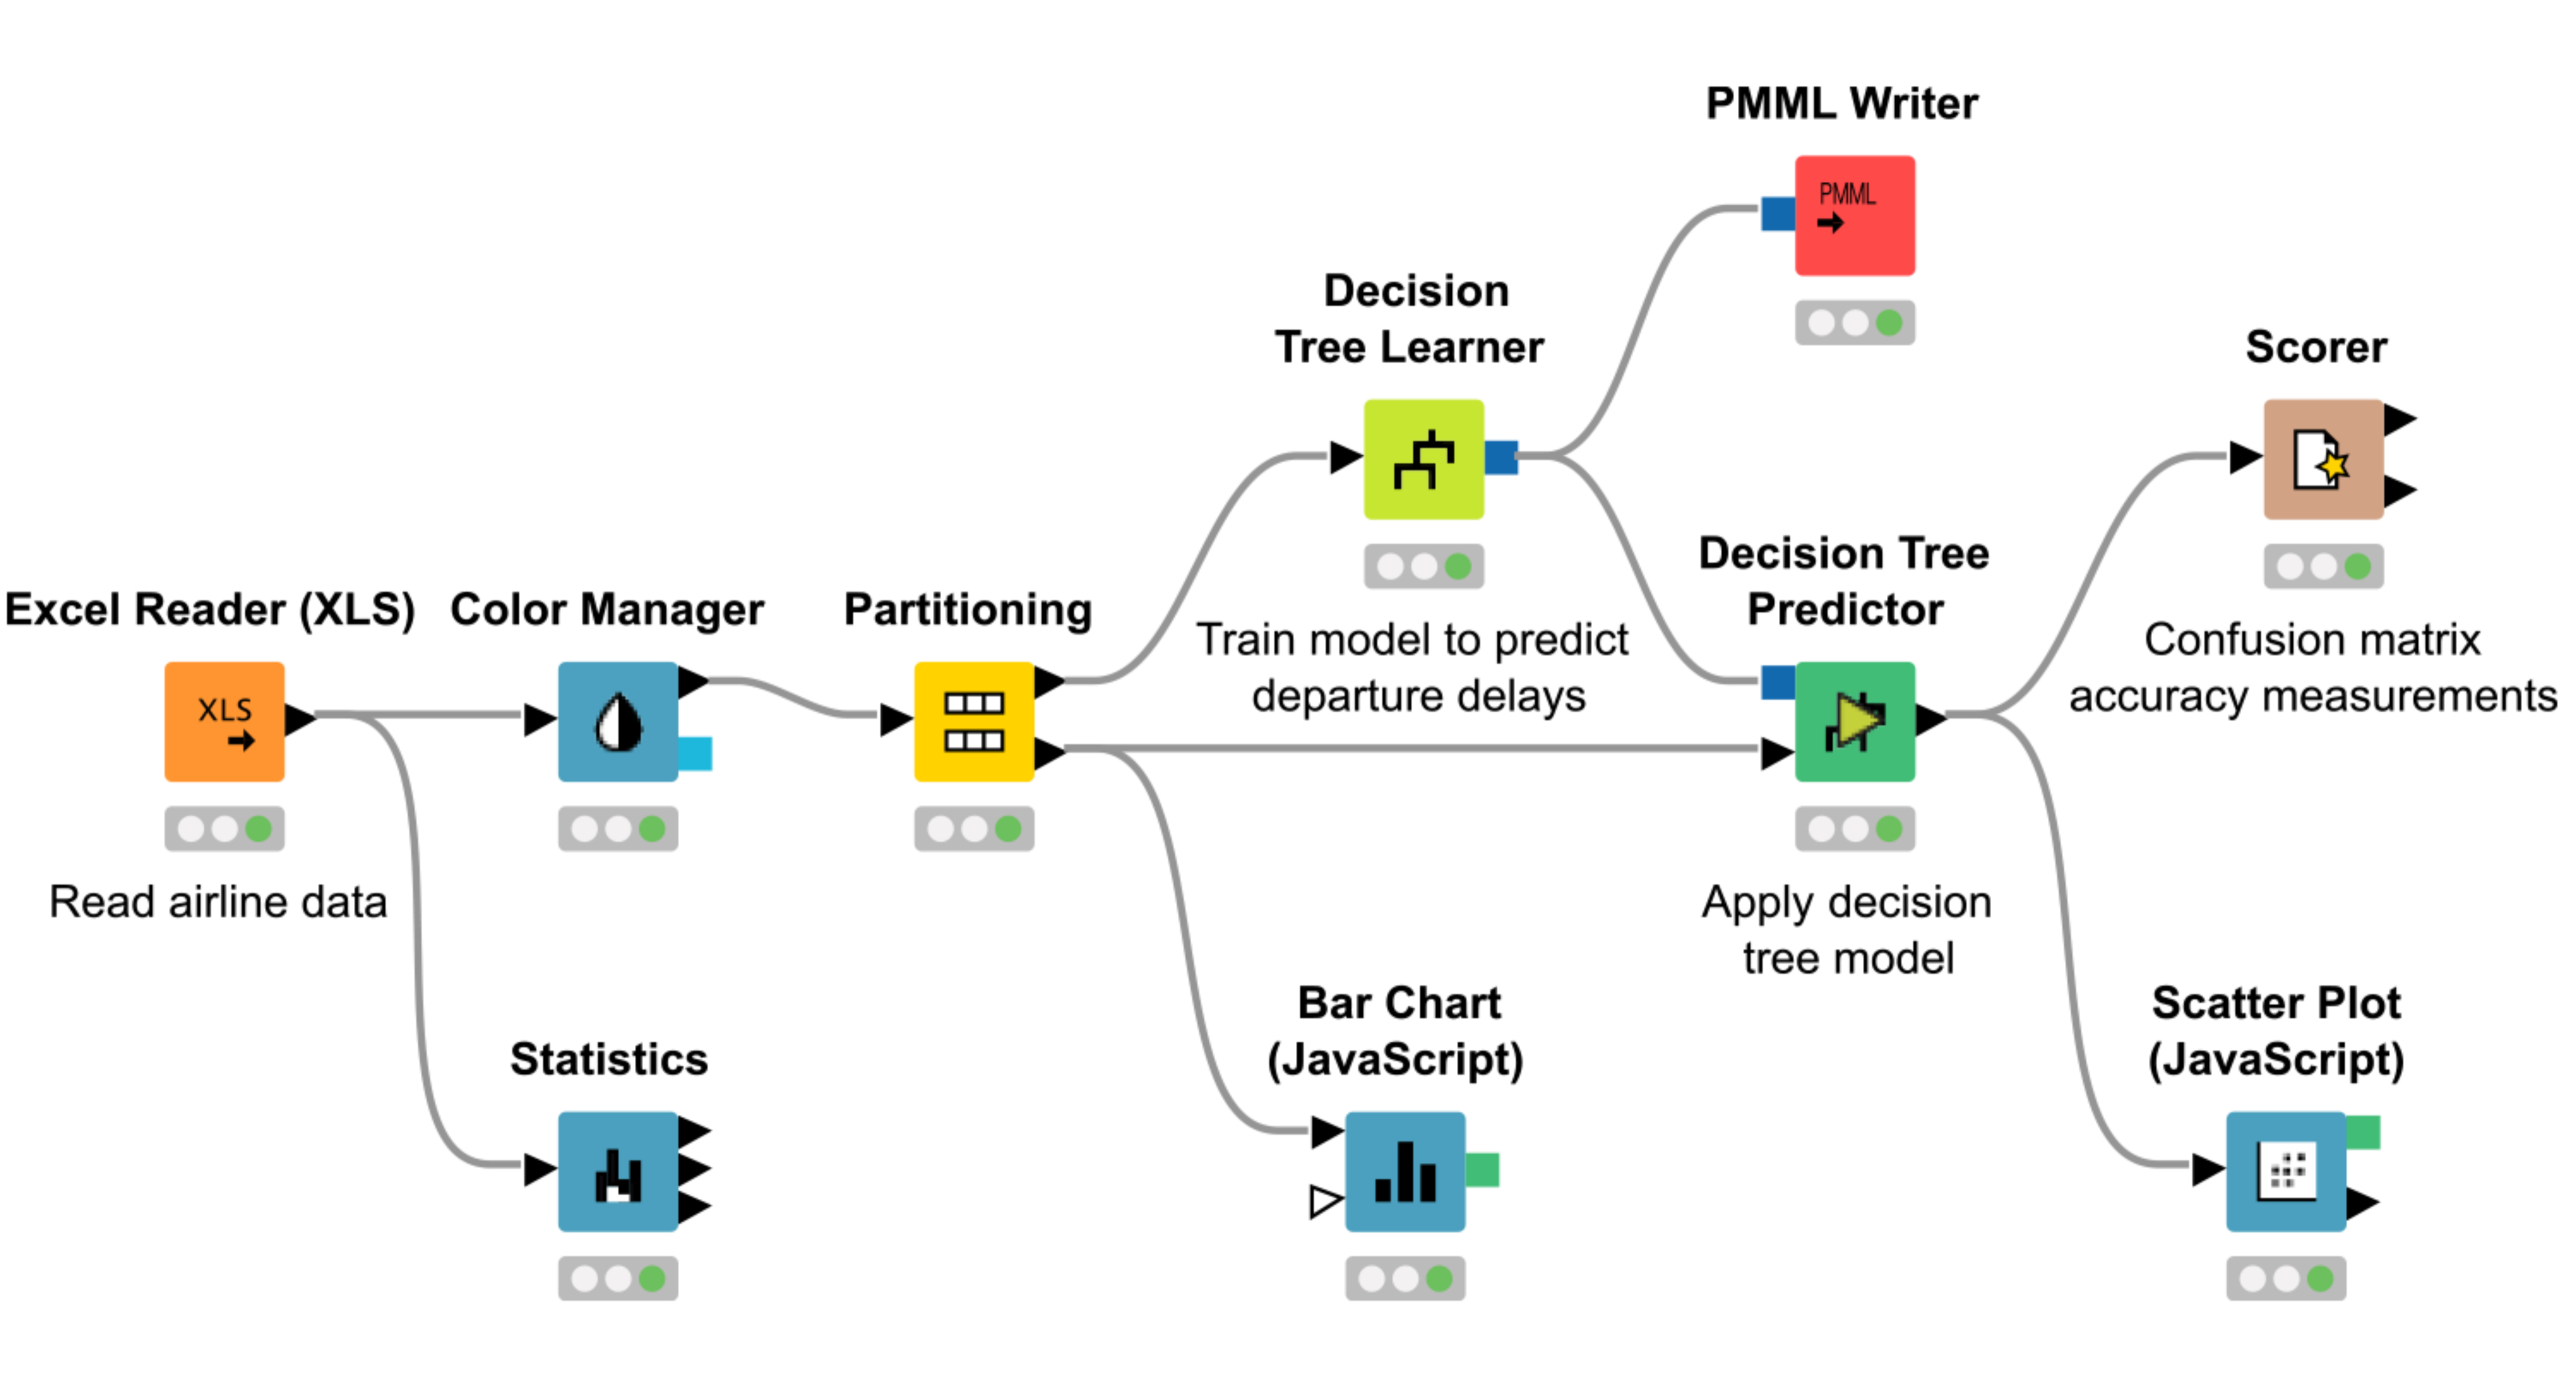
\includegraphics[width=400pt]{nocode-data.png}
\caption{An examples of a data analysis workflow created using the KNIME IDE}
\end{figure}

The approach depicted so far goes under the name of no-code programming since there is coding logic involved, only relations between entities. Although this approach works for workflow definition, there could be more complex manipulation that require a coding approach. For these cases, it is still possible to rely on a visual approach that goes under the name of low-code. 
\begin{figure}
\label{lowcode}
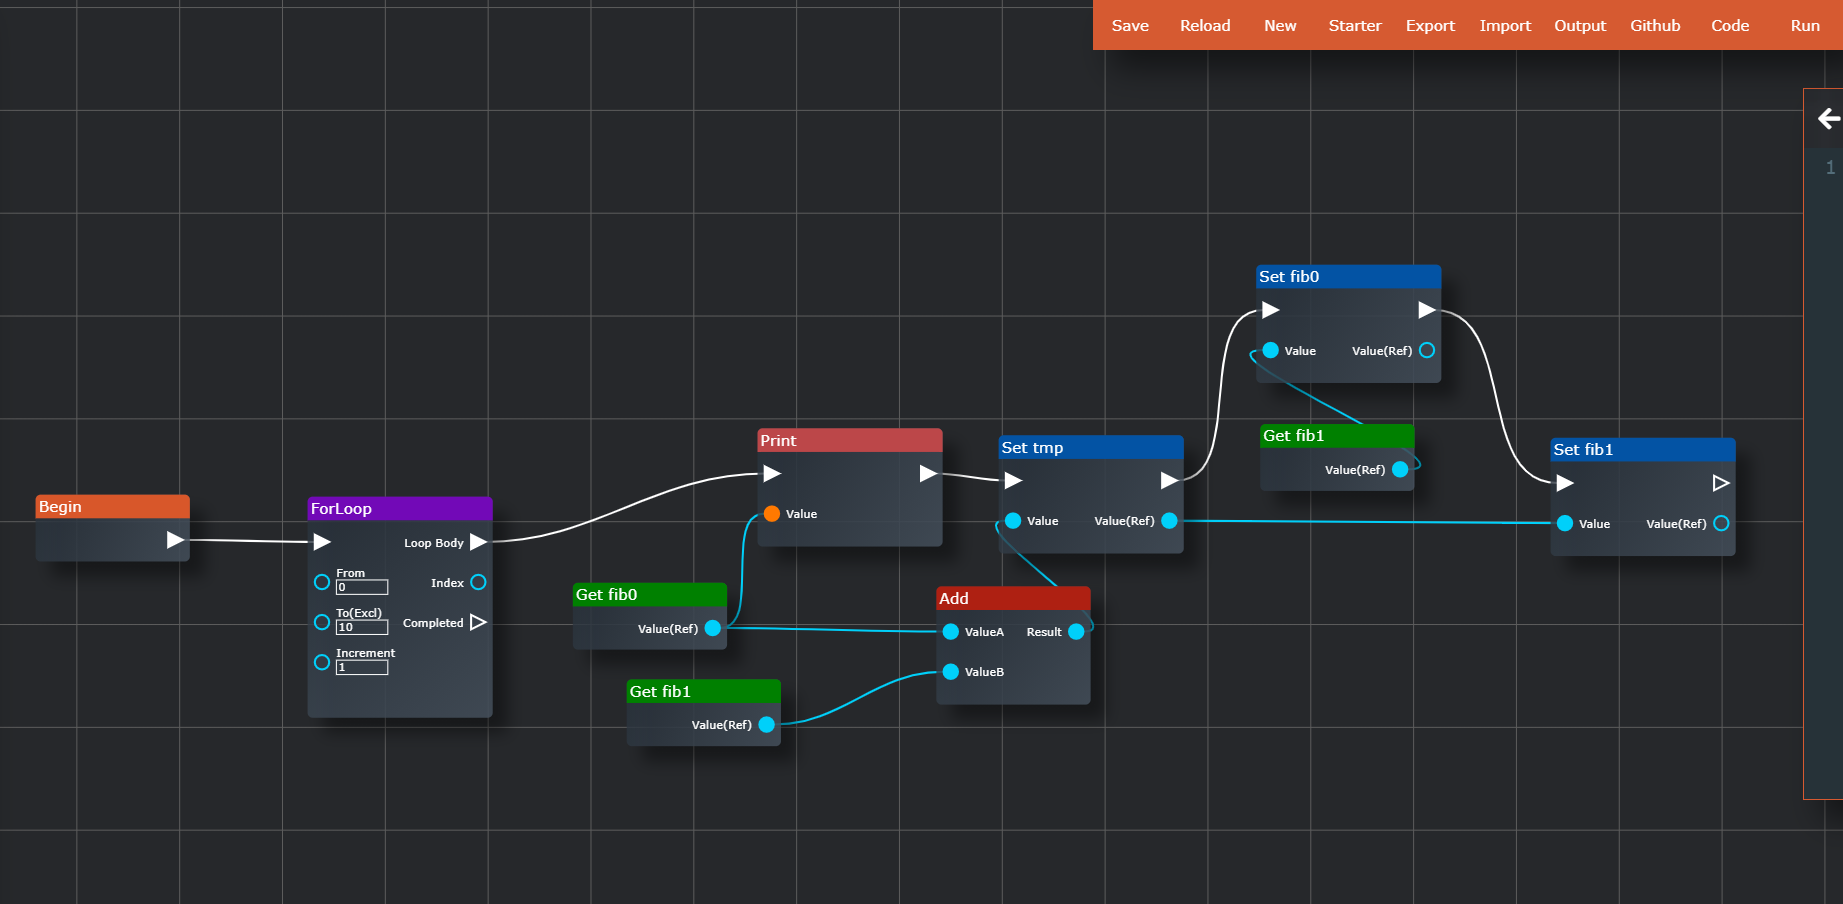
\includegraphics[width=400pt]{lowcode.png}
\caption{An examples of a Fibonacci sequence in CodeWire}
\end{figure}
Fig. \ref{lowcode} shows an example of a piece of code that generates the Fibonacci sequence, written in CodeWire. While retaining the logic and control structure of a programming language, it abstracts the details of the specific programming language. 

The approach we want pursue in the PoC platform for dealii-X should sport both strategies, allowing high-level control by means of the no-code interface, while retaining the possibility of deep customization through the low-code interface. 

This will be achieved by allowing user to define their custom no-code nodes in term of low-code logic.

The rest of the deliverable is organized as follows: in section 2 we sketch the low-code approach with a practical example using the dealii library. In section 3 we sketch instead the no-code approach to the simulation, using the nodes defined in section 2. In section 3 we outline the devolvement plan of PoC and the relative improvments we envision. 


\section{\textcolor{EUblue}{Low-code approach to dealii programming}}

In the present section we go on the details of the design of a node-based low-code interface for an Object Oriented Library, using dealii as an operative example.

A minimal set of entiies and control loop that allow the creation of an object-oriented, Turing-complete language is the following:
\begin{itemize}
\item Variables and instances of objects
\item Functions and member functions
\item Loops
\item Conditionals
\end{itemize}

Each of these entities can be represented as a node in a graph, with inputs and outputs. The graph is then traversed in a way that is consistent with the logic of the programming language.

For a example, a basic type like int can be represented, as shown in fig.\ref{sum}, as a node with a single output pin. The sum is then represented as a node with two input pins and one output pin. 

\begin{figure}
    \label{sum}
    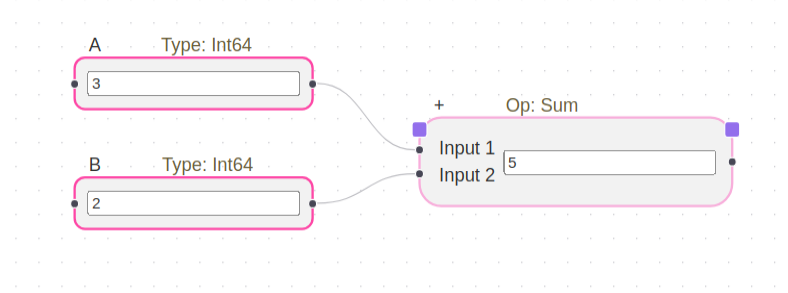
\includegraphics[width=400pt]{sum.png}
    \caption{Node-based mockup of a sum operation}
\end{figure}

To specify order of the operation, special connectors one the node are used, and special edges are display, to distinguish instruction flow from arguments. For example, su subsequent sums would look like (fig.\ref{twosum}).

\begin{figure}
    \label{twosum}
    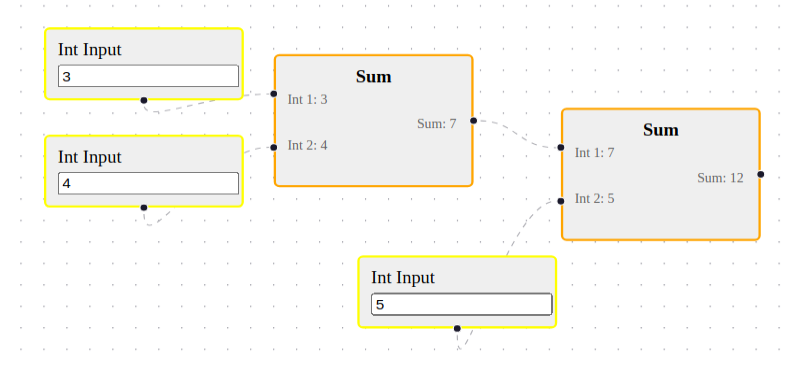
\includegraphics[width=400pt]{twosum.png}
    \caption{Node-based mockup of a two subsequent sum operations}
\end{figure}
    

Object work in the same way, but member functions nodes can be attached to the object instance node, and the output of the function can then be passed to other nodes.

Fig. \ref{refine} shows an example of a node-based representation of a mesh refinement operation in dealii. The mesh is read from a file, and then refined, calling generic function and member functions of the mesh object.
\begin{figure}
    \label{refine}
    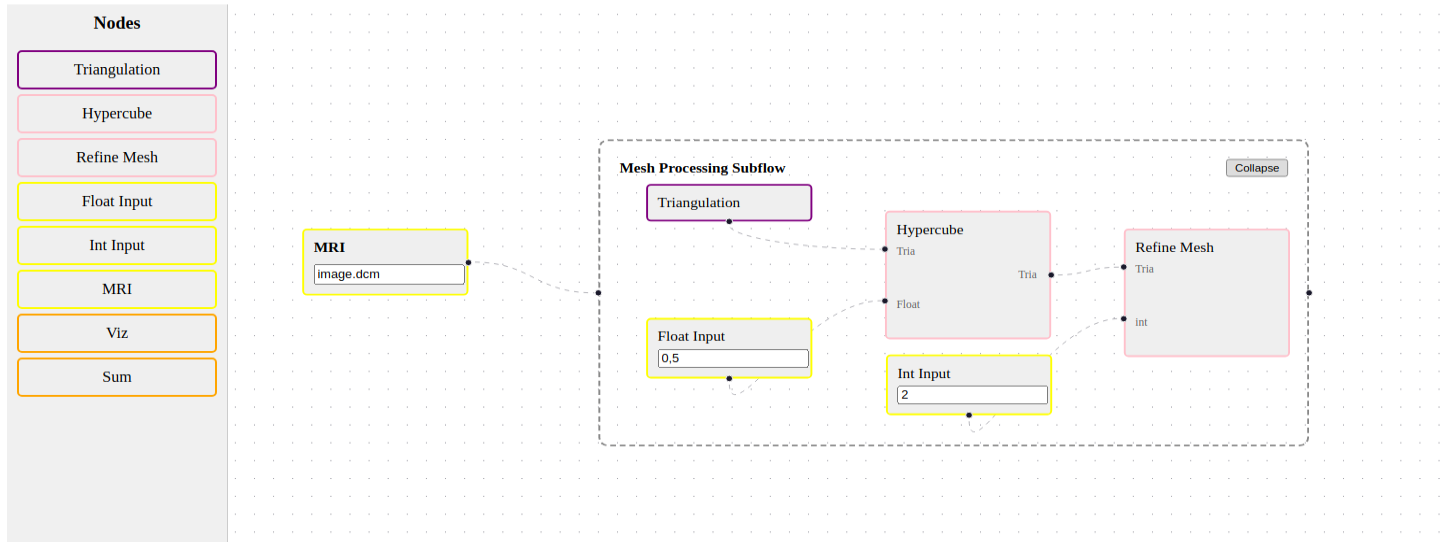
\includegraphics[width=400pt]{refine.png}
    \caption{Node-based mockup of a mesh refinement operation}
\end{figure}


The power of node-based programming is twofold: on one side, it allows to create complex operations without knowing the details of a specific programming language. On the other side, it allows to encapsulate a collection of nodes into a single node, that can be reused in other parts of the program. This hierarchical features unleash the possibility of creating high level entities that can be used by non-expert users. The latter is the key feature that links the low-code and no-code approach, allowing the creation of a single environment that can be used by both expert and non-expert users.

Moreover, the node-based approach naturally leads to the definition of a computational graph, that can be used to optimize the execution of the program: by analizing the graph, it is possible to determine which parts of it can be executed concurrently, which allows a potential second layer of parallelization on top of the one that is already present in the libraries. Operatively, we are currently investigating the use of the \href{https://github.com/taskflow/taskflow}{taskflow} library to implement graph analysis and node scheduling.   

\section{\textcolor{EUblue}{No-code approach to simulation management}}

As noted in the previous section, given the hierarchical nature of node-based programming, it is possible to create high-level entities that completely hide the technical details, while still allowing the creation of complex dataflow. For example, the simulation block defined in fig.\ref{nocode-sim} can be encapsulated in a single, opaque node, that only requires e.g. an MRI input and a place to display the results. 

\begin{figure}
    \label{nocode-sim}
    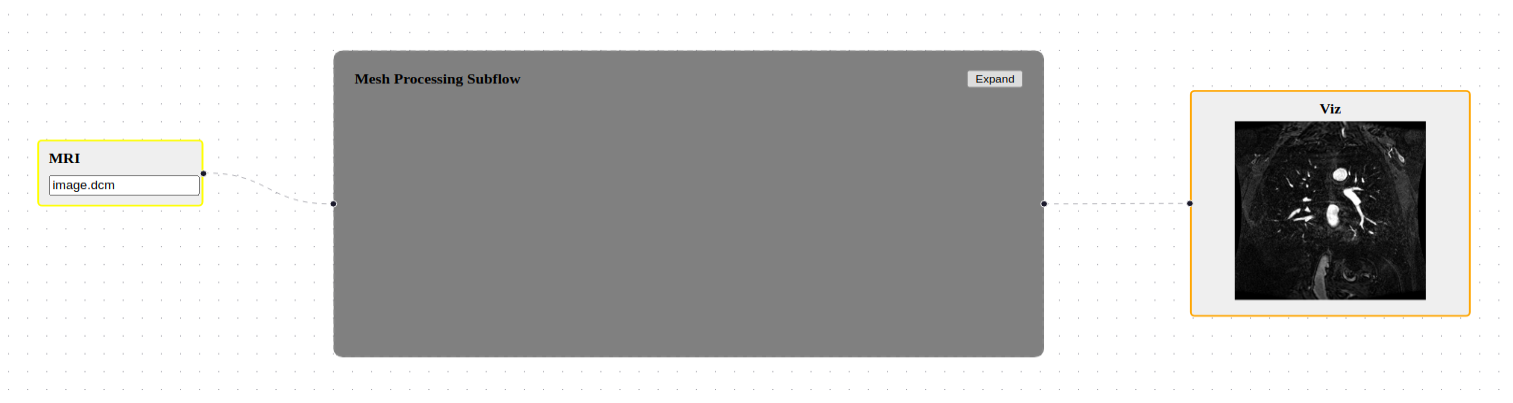
\includegraphics[width=400pt]{nocode-sim.png}
    \caption{Mockup of the high level no-code interaction}
\end{figure}



This high level view of the computational workflow will also allow the quick selection of the computational resource to be used, abstracting the details of different HPC or cloud systems. This system, which will be calling "metascheduler", will be developed in the context of the dealii-X project, and will be used to manage the computational resources of the PoC platform.

The entire platform, from the low-code interface to the metascheduler, will be served by means of a webapp, that will allow the user to interact with the system from any device, and will be developed using the latest web technologies. 

\section{\textcolor{EUblue}{PoC development plan and outlook}}

The main development activities for the PoC platform are the following will be carried out in task 2.6.2 and 2.6.3. The development activities will start in M7, with main frontend and backend of the low-code/no-code PoC platform being developed concurrently. The low-code system will be agnostic of the underling simulation library used, in order to easily integrate the progess of the various dealii-X libraries for specific organs. The activities on the metascheduler will start in M7 as well. Both the low-code/no-code interface and the metascheduler will be developed in an iterative way, with the first version of the PoC platform being deployed in M17. Between M18 anb month M22 the PoC platform will be tested by the partners, and the feedback will be used to improve the platform in the following months. The final tranche of the development will be between M23 and M27, in which the final version of the PoC platform will be deployed.

The Gantt chart of the activities is shown in fig.\ref{gannt}. The frontend of the PoC platform will be in charge of Dualistic, while the backend and the metascheduler will be developed by eXact lab. The activitis will be carried out in close collaboration with the other partners of the dealii-X project, UniPI in particular. 
\begin{figure}
    \label{gannt}
    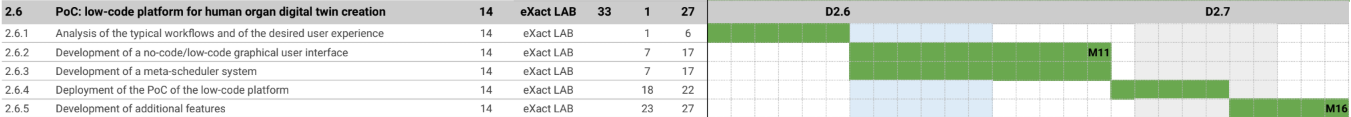
\includegraphics[width=400pt]{gantt.png}
    \caption{Timeline of the activities of task 2.6, Creation of the PoC platform}
\end{figure}
The PoC platform is forseseen to be a valuable exploitable result of the dealii-X project, and will be used to showcase the capabilities of the libraries developed in the project.

\label{MyLastPage}


\end{document}
